\section{使用导数的最优化方法}
\textbf{最速下降法、牛顿法、共轭梯度法}、拟牛顿法、信赖域法、最小二乘法.

\subsection{最速下降法}
\begin{note}
    最速下降法,$f(x)$ 具有一阶连续偏导数 \[\begin{cases}
        \min \quad &f(x)\\
        \subject \quad &x \in E^n
    \end{cases}\]
    带精确线搜索的最速下降法 \begin{enumerate}
        \item 给定初始点 $x^{(1)} \in E^n$,允许误差 $\varepsilon > 0$,置 $k = 1$.
        \item 取搜索方向:$d^{(k)} = -\nabla f(x^{(k)})$
        \item 若 $\norm{d^{(k)}} \le \varepsilon$,则停止计算;否则,从 $x^{(k)}$ 出发,沿 $d^{(k)}$ 进行一维搜索,求 $\lambda_k$,使 \[f(x^{(k)} + \lambda_k d^{(k)}) = \min_{\lambda \ge 0} f(x^{(k)} + \lambda d^{(k)})\]
        \item 令 $x^{(k + 1)} = x^{(k)} + \lambda_k d^{(k)}$,置 $k := k + 1$,返回2
    \end{enumerate}
\end{note}

\begin{example}
    求 $\min f(x) = (x_1 - 1)^2 + (x_2 - 1)^2$,取 $x^{(1)} = (0, 0)^t, \varepsilon = 1e-5$
    \answer $\nabla f(x) = (2(x_1 - 1), 2(x_2 - 1))^t$

    第一次迭代\begin{itemize}
        \item $d^{(1)} = -(-2, -2)^t = (2, 2)^t, \norm{d^{(1)}} = 2\sqrt{2} > \varepsilon$
        \item $\underset{\lambda \ge 0}{\min} \varphi(\lambda) = \underset{\lambda \ge 0}{\min} f(x^{(1)} + \lambda d^{(1)})$,得 $\lambda = \frac{1}{2}$.
        \item $x^{(2)} = x^{(1)} + \lambda d^{(1)} = (1, 1)^t$
    \end{itemize}
    第二次迭代\begin{itemize}
        \item $d^{(2)} = (0, 0)^t, \norm{d} = 0 < \varepsilon$
    \end{itemize}
    故 $(1, 1)^t$ 为最优解.
\end{example}

\begin{note}
    最速下降法(二次情形):对任意 $x^{(0)} \in E^n$,最速下降法产生得序列收敛于 $f(x)$ 的唯一极小点 $x^*$,而且,对任意的 $k$,有\[E(x^{(k + 1)}) \le \left(\frac{A - a}{A + a}\right)E(x^{(k)})\] 其中 $E(x) = \frac{1}{2}(x - x^*)^tQ(x - x^*)$,$A$ 为 $f(x)$ 的Hesse矩阵的最大特征值,$a > 0$ 为最小特征值.

    最速下降法(非二次情形):设 $f(x)$ 存在连续二阶偏导数,$\bar{x}$ 是局部极小点,Hesse矩阵 $\nabla^2f(\bar{x})$ 的最小特征值 $a > 0$,最大特征值为 $A$,算法产生的序列 $\{x^{(k)}\}$ 收敛于点 $\bar{x}$,则目标函数值的序列 $\{f(x^{(k)})\}$ 以不大于 $\left(\frac{A - a}{A + a}\right)^2$ 的收敛比线性的收敛于 $f(\bar{x})$. 令条件数 $r = \frac{A}{a}$,则 $\left(\frac{A-a}{A+a}\right)^{2}=\left(\frac{r-1}{r+1}\right)^{2}<1$.
\end{note}

\begin{note}
    在相继两次迭代中,梯度方向互相正交.
    \begin{proof}
        令 $\varphi(\lambda) = f(x^{(k)} + \lambda d^{(k)}), d^{(k)} = -\nabla f(x^{(k)})$,为求出从 $x^{(k)}$ 出发沿方向 $d^{(k)}$ 的极小点,令 \[\varphi^\prime(\lambda_k) = \nabla f(x^{(k)} + \lambda_kd^{(k)})^td^{(k)} = 0\] 得 $-\nabla f(x^{(k + 1)})^t\nabla f(x^{(k)}) = 0$,即方向 $d^{(k + 1)} = -\nabla f(x^{(k + 1)})$ 与 $d^{(k)} = -\nabla f(x^{(k)})$ 正交.
    \end{proof}
\end{note}

\subsection{牛顿法}
\begin{note}
    牛顿法计算步骤:\begin{enumerate}
        \item 给定初始点 $x^{(0)} \in E^n$,允许误差 $\varepsilon > 0$,置 $k = 0$
        \item 若 $\norm{\nabla f(x^{(k)})} < \varepsilon$,则停止计算;
        \item $x^{(k + 1)} = x^{(k)} - \left(\nabla^2f(x^{(k)})\right)^{-1}\nabla f(x^{(k)})$,置 $k:=k + 1$,返回2.
    \end{enumerate}
\end{note}

\begin{example}
    求 $\min f(x) = x_1^2 + 25x_2^2$
    \answer $\nabla f = \begin{pmatrix}
        2x_1\\ 50x_2
    \end{pmatrix}, \nabla^2f = \begin{pmatrix}
        2 & 0 \\ 0 & 50
    \end{pmatrix}$
    
    取 $x^{(0)} = (2, 2)^t$,$x^{(1)} = x^{(0)} - \nabla^2f(x^{(0)})^{-1}\nabla f(x^{(0)}) = (0, 0)^t$. 
    
    $\norm{\nabla f(x^{(1)})} = 0$,则 $x^* = (0, 0)$.
\end{example}

\begin{note}
    牛顿迭代法的缺点:\begin{enumerate}
        \item 可能会出现某步迭代时,目标函数值上升
        \item 当初始点远离极小点时,牛顿法产生的点列可能不收敛,或者收敛到鞍点,或者Hesse矩阵不可逆,无法计算
        \item 需要计算Hesse矩阵,计算量大
    \end{enumerate}
    牛顿迭代法的优点:\begin{enumerate}
        \item 产生的点列 $\{x^{(k)}\}$ 若收敛,则收敛速度快,具有至少二阶收敛速率.
        \item 牛顿法具有二次终止性(正定二次函数可以一次迭代到达最优点).
    \end{enumerate}
\end{note}

\begin{note}
    阻尼牛顿法计算步骤:\begin{enumerate}
        \item 给定初始点 $x^{(1)} \in E^n$,允许误差 $\varepsilon > 0$,置 $k = 1$
        \item 计算 $\nabla f(x^{(k)}), \nabla^2f(x^{(k)})^{-1}$
        \item 若 $\norm{\nabla f(x^{(k)})} < \varepsilon$,则停止迭代;否则,令 $d^{(k)} = \nabla^2f(x^{(k)})^{-1}\nabla f(x^{(k)})$
        \item 从 $x^{(k)}$ 出发,沿方向 $d^{(k)}$ 作一维搜索:\[\min_{\lambda} f(x^{(k)} + \lambda d^{(k)}) = f(x^{(k)} + \lambda_k d^{(k)})\] 令 $x^{(k + 1)} = x^{(k)} + \lambda_k d^{(k)}$
        \item 置 $k := k + 1$,转步骤2.
    \end{enumerate}
\end{note}

\begin{note}
    修正牛顿法计算步骤:\begin{enumerate}
        \item 给定初始点 $x^{(1)} \in E^n$,允许误差 $\varepsilon > 0$,置 $k = 1$
        \item 计算 $\nabla f(x^{(k)}), \nabla^2f(x^{(k)})^{-1}$
        \item 若 $\norm{\nabla f(x^{(k)})} < \varepsilon$,则停止迭代;否则,置 $B_k = G_k + \varepsilon_k I$,其中 $\varepsilon_k$ 是一个非负数,选取 $\varepsilon_k$,使得 $B_k$ 是对称正定矩阵,计算修正牛顿方向 $d^{(k)} = -B_k^{-1}\nabla f(x^{(k)})$
        \item 从 $x^{(k)}$ 出发,沿方向 $d^{(k)}$ 作一维搜索:\[\min_{\lambda} f(x^{(k)} + \lambda d^{(k)}) = f(x^{(k)} + \lambda_k d^{(k)})\] 令 $x^{(k + 1)} = x^{(k)} + \lambda_k d^{(k)}$
        \item 置 $k := k + 1$,转步骤2.
    \end{enumerate}
\end{note}

\begin{note}
    牛顿-最速下降法计算步骤:\begin{enumerate}
        \item 给定初始点 $x^{(1)} \in E^n$,允许误差 $\varepsilon > 0$,置 $k = 1$
        \item 计算 $g_k = \nabla f(x^{(k)})$. 若 $\norm{g_k} \le \varepsilon$,算法终止,输出 $x^{(k)}$ 作为近似最优解;否则,转步骤3
        \item 计算 $G_k = \nabla^2f(x^{(k)})$. 解线性方程组\[G_kd^{(k)} + \nabla f(x_k) = 0\] 若有解 $d^{(k)}$ 且满足 $g_k^td^{(k)} < 0$,转步骤4,否则令 $d^{(k)} = -g_k$,转步骤4
        \item 从 $x^{(k)}$ 出发,沿方向 $d^{(k)}$ 作一维搜索:\[\min_{\lambda} f(x^{(k)} + \lambda d^{(k)}) = f(x^{(k)} + \lambda_k d^{(k)})\] 令 $x^{(k + 1)} = x^{(k)} + \lambda_k d^{(k)}$
        \item 置 $k := k + 1$,转步骤2.
    \end{enumerate}
\end{note}

\subsection{共轭梯度法}
\begin{note}
    共轭方向:设 $A$ 是 $n \times n$ 对称正定矩阵,若 $E^n$ 中的两个方向 $d^{(1)}$ 和 $d^{(2)}$ 满足 $(d^{(1)})^tAd^{(2)} = 0$,则称这两个方向关于 $A$ 共轭,或称它们关于 $A$ 正交.

    若 $d^{(1)}, \dots, d^{(k)}$ 是 $E^n$ 中 $k$ 个方向,它们两两关于 $A$ 共轭,即 $(d^{(1)})^tAd^{(2)} = 0, i \neq j$,则称这组方向是 $A$ 共轭的,或称它们为 $A$ 的 $k$ 个共轭方向.
\end{note}

\begin{theorem}
    设 $A$ 是 $n$ 阶对称正定矩阵,$d^{(1)}, \dots, d^{(k)}$ 是 $k$ 个 $A$ 共轭的非零向量,则这 $k$ 个向量线性无关.
    \begin{proof}
        对于正定矩阵 $A$,$\alpha_{1} d^{(1)}+\alpha_{2} d^{(2)}+\cdots+\alpha_{k} d^{(k)}=0$ 必有 $\alpha_i = 0$.
    \end{proof}
\end{theorem}

\begin{theorem}
    二次函数 $f(x) = \frac{1}{2}x^tAx + b^tx + c$,其中 $A_{n \times n}$ 是对称正定矩阵,$d^{(1)}, \dots, d^{(n - 1)}$ 是 $A$ 共轭的非零向量,从任意一点 $x^{(0)} \in E^n$ 出发,依次沿这组向量进行一维搜索\[\underset{\lambda \ge 0}{\min} f(x^{(k)} + \lambda d^{(k)})\]$x^{(k + 1)} = x^{(k)} + \lambda_k d^{(k)}, k = 0, \dots, n - 1$,则 $\nabla f(x^{(k + 1)})^t d^{(j)} = 0, j = 0, \dots, k$,即搜索方向和之前所有的搜索方向都正交,并且最多经过 $n$ 步收敛.
\end{theorem}

\begin{note}
    记 $g_i = \nabla f(x^{(i)})$

    FR共轭梯度法(二次凸函数)\begin{enumerate}
        \item 给定初始点 $x^{(1)}$,置 $k = 1$
        \item 计算 $g_k = \nabla f(x^{(k)})$,若 $\norm{g_k} = 0$,则停止计算,否则进行下一步
        \item 令 $d^{(k)} = -g_k + \beta_{k - 1}d^{(k - 1)}$,其中,当 $k = 1$ 时,$\beta_0 = 0$,当 $k > 1$ 时,$\beta_{k - 1} = \frac{d^{(k - 1)t}Ag_k}{d^{(k - 1)t}Ad^{(k - 1)}} = \frac{\norm{g_k}^2}{\norm{g_{k - 1}}^2}$
        \item 令 $x^{(k + 1)} = x^{(k)} + \lambda_kd^{(k)}$,其中 $\lambda_k = \frac{g_k^tg_k}{d^{(k)t}Ad^{(k)}}$
        \item 若 $k = n$,则停止计算,否则置 $k = k + 1$,返回步骤2.
    \end{enumerate}
\end{note}

\begin{theorem}
    对正定二次函数,FR法在 $m \le n$ 次一维搜索后终止,且对 $\forall i(1 \le i \le m)$,下列关系成立
    \begin{enumerate}
        \item $d^{(i)t}Ad^{(j)} = 0, j = 1, \dots, i - 1$
        \item $g_i^tg_j = 0, j = 1, \dots, i - 1$
        \item $g_i^td^{(i)} = -g_i^tg_i$
    \end{enumerate}
\end{theorem}

\begin{note}
    一般函数的共轭梯度法\begin{enumerate}
        \item 步长 $\lambda_k$ 不能再用公式 $\lambda_k = -\frac{g_k^tg_k}{d^{(k)t}Ad^{(k)}}$ 计算,必须用其他一维搜索方法来确定
        \item 凡用到矩阵 $A$ 之处,需用现行点的Hession矩阵 $\nabla^2f(x^{(k)})$ 代替
        \item 有限步迭代达不到极小点
    \end{enumerate}
\end{note}

\begin{figure}[htbp]
    \centering
    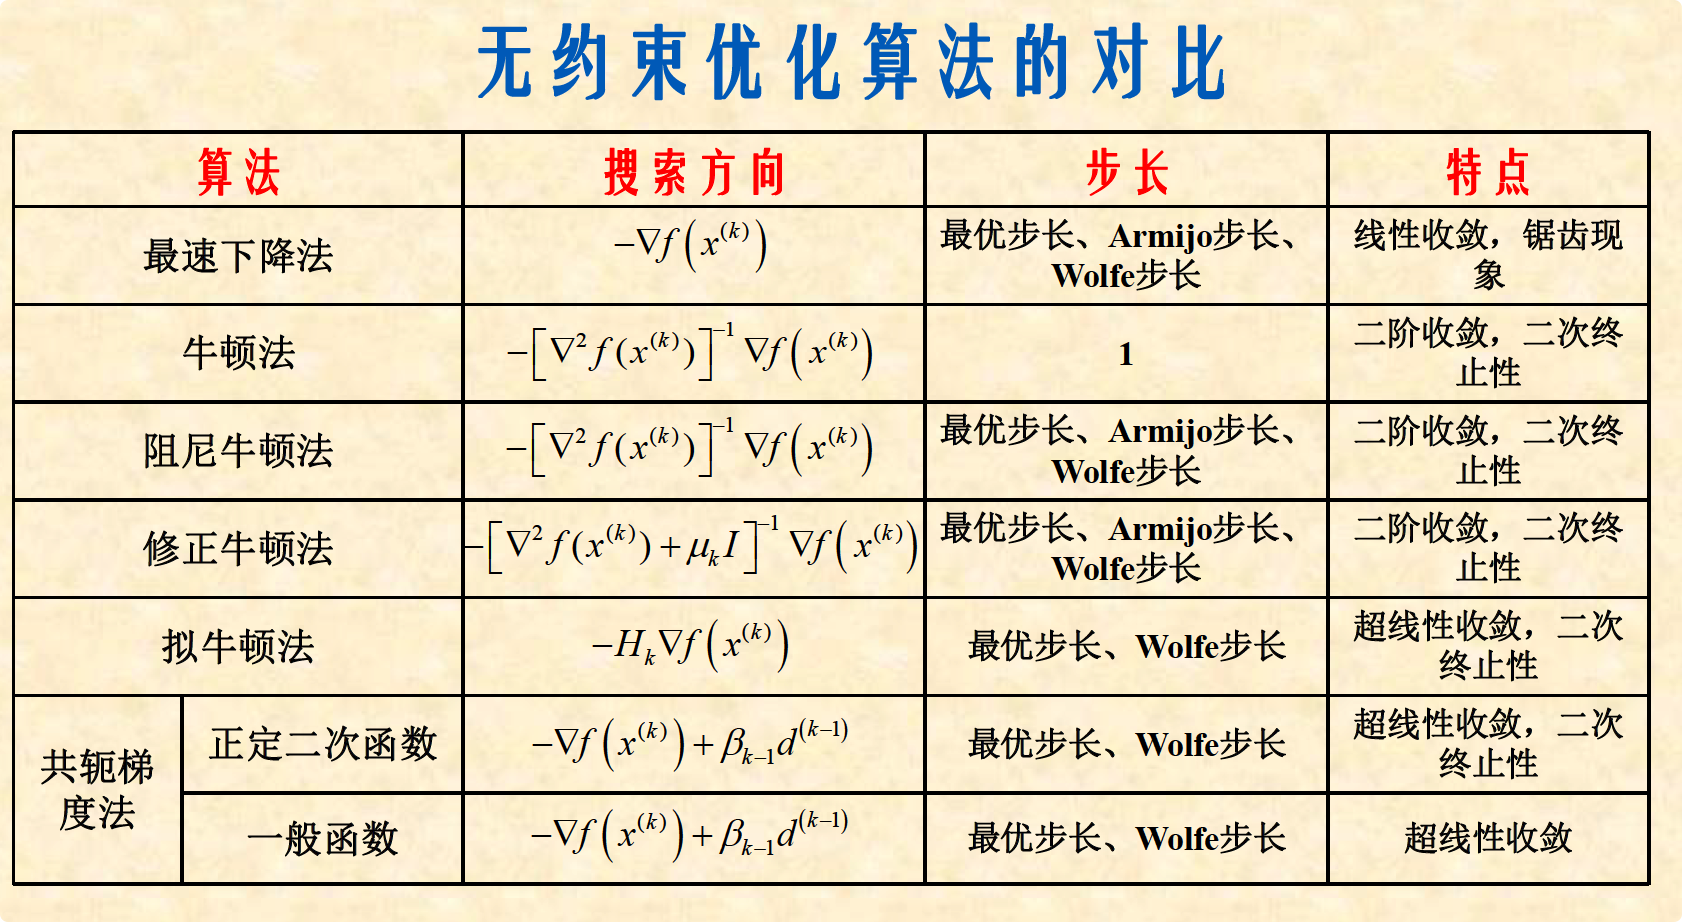
\includegraphics[width=0.8\textwidth]{./figures/img3.png}
    \caption{无约束优化算法的对比 \label{fig3}}
\end{figure}
